In this section, the theoretical model of \textit{SA}~\cite{Collins_Loftus_1975,AndersonTheory} is reviewed to 
illustrate the basic components and the operations performed by SA during their execution, specially
the spread of the activation from a node to their adjacent, see Fig.~\ref{fig:spreading}. 
This model is made up of a conceptual network of nodes connected through relations (conceptual graph). 
Taking into account that nodes represent domain objects or classes and edges relations among them, 
it is possible to establish a semantic network in which SA can be applied. The process performed by the algorithm 
is based on a thorough method to go down the graph using an iterative model. Each iteration is comprised of 
a set of beats, a stepwise method, and the checking of a stop condition. 
Following the different stages of SA are presented and defined:

\begin{figure}[h]
 \centering
    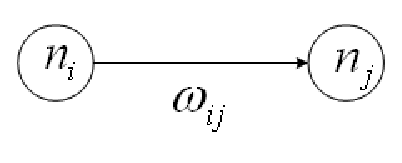
\includegraphics[width=3cm]{images/spreading}
    \caption{Graphical model of \textit{Spreading Activation}}
 \label{fig:spreading}
\end{figure}

\begin{description}
\item [\textit{Preadjustement}:] This is the initial and optional stage. It is usually in charge
of performing some control strategy over the target semantic network.
\medskip

\item [\textit{Spreading}:] This is the spread stage of the algorithm. Concepts
are activated in activation waves. The spreading node activates its neighbor
nodes, see Fig.~\ref{fig:modelo-sa}.
\medskip

The calculation of the activation rank $I_i$ of a node $n_i$ is defined as
follows:

\begin{equation}
I_i  = \sum_j{O_j \omega_{ji}}
\end{equation}
\medskip

$I_i$ is the total inputs of the node $n_i$, $O_j$
is the output of the node $n_j$ connected to $n_i$ and $\omega_{ji}$
is the weight of the relation between $n_j$ and $n_i$. 
If there is not relation between $n_j$ and $n_i$ then
$\omega_{ji} = 0$. 


The activation function $f$ is used to evaluate the ``weight'' of a node and
decide if the concept is active.


\begin{equation}
N_i=f(I_i)=\begin{cases} 0 & \text{if $I_i < \jmath_i$} \\ 1 &
\text{if $I_i > \jmath_i$}
\\ \end{cases}
\end{equation}


$N_i$ is $1$ if the node has been activated or 0 otherwise. 
$\jmath_i$, the threshold activation value for node $i$, depends on the application
and it can change from a node to others. The activation rank $I_i$ of a
node $n_i$ will change while algorithm iterates.

\begin{figure}[h]
 \centering
 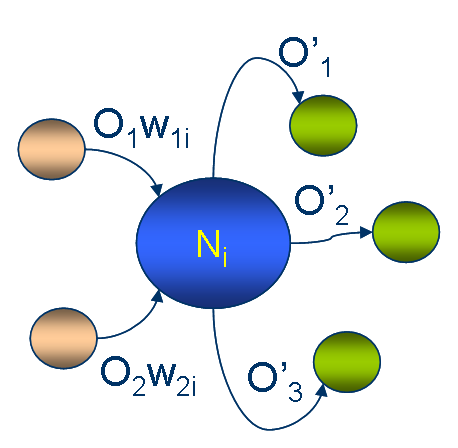
\includegraphics[width=4cm]{images/modelo-sa}
    \caption{Activation of concepts in \textit{Spreading Activation}}
 \label{fig:modelo-sa}
\end{figure}

\item [\textit{Postadjustment}:] This is the final and optional stage. As well as
\textit{Preadjustment} stage, it is used to perform some control strategy in the
set of activated concepts.

\end{description}
